%%% Hlavní soubor. Zde se definují základní parametry a odkazuje se na ostatní části. %%%

%% Verze pro jednostranný tisk:
% Okraje: levý 40mm, pravý 25mm, horní a dolní 25mm
% (ale pozor, LaTeX si sám přidává 1in)
\documentclass[12pt,a4paper]{report}
\setlength\textwidth{145mm}
\setlength\textheight{247mm}
\setlength\oddsidemargin{15mm}
\setlength\evensidemargin{15mm}
\setlength\topmargin{0mm}
\setlength\headsep{0mm}
\setlength\headheight{0mm}
% \openright zařídí, aby následující text začínal na pravé straně knihy
\let\openright=\clearpage

%% Pokud tiskneme oboustranně:
% \documentclass[12pt,a4paper,twoside,openright]{report}
% \setlength\textwidth{145mm}
% \setlength\textheight{247mm}
% \setlength\oddsidemargin{14.2mm}
% \setlength\evensidemargin{0mm}
% \setlength\topmargin{0mm}
% \setlength\headsep{0mm}
% \setlength\headheight{0mm}
% \let\openright=\cleardoublepage

%% Vytváříme PDF/A-2u
\usepackage[a-2u]{pdfx}
\usepackage{listings}
\def\inline{\lstinline[basicstyle=\ttfamily,keywordstyle={}]}

%% Přepneme na českou sazbu a fonty Latin Modern
\usepackage[czech]{babel}
\usepackage{lmodern}
\usepackage[T1]{fontenc}
\usepackage{textcomp}

%% Použité kódování znaků: obvykle latin2, cp1250 nebo utf8:
\usepackage[utf8]{inputenc}

%%% Další užitečné balíčky (jsou součástí běžných distribucí LaTeXu)
\usepackage{amsmath}        % rozšíření pro sazbu matematiky
\usepackage{amsfonts}       % matematické fonty
\usepackage{amsthm}         % sazba vět, definic apod.
\usepackage{bbding}         % balíček s nejrůznějšími symboly
			    % (čtverečky, hvězdičky, tužtičky, nůžtičky, ...)
\usepackage{bm}             % tučné symboly (příkaz \bm)
\usepackage{graphicx}       % vkládání obrázků
\usepackage{fancyvrb}       % vylepšené prostředí pro strojové písmo
\usepackage{indentfirst}    % zavede odsazení 1. odstavce kapitoly
\usepackage{natbib}         % zajištuje možnost odkazovat na literaturu
			    % stylem AUTOR (ROK), resp. AUTOR [ČÍSLO]
\usepackage[nottoc]{tocbibind} % zajistí přidání seznamu literatury,
                            % obrázků a tabulek do obsahu
\usepackage{icomma}         % inteligetní čárka v matematickém módu
\usepackage{dcolumn}        % lepší zarovnání sloupců v tabulkách
\usepackage{booktabs}       % lepší vodorovné linky v tabulkách
\usepackage{paralist}       % lepší enumerate a itemize

%%% Údaje o práci

\def\NazevSkoly{Gymnázium, Praha 6, Arabská 14}
% Název oboru včetně počátečního 'Obor'.
\def\NazevOboru{Obor programování}

% Název práce v jazyce práce (přesně podle zadání)
\def\NazevPrace{<NazevPrace>}

% Název práce v angličtině
\def\NazevPraceEN{<NazevPraceEN>}

% Jména autorů
% Abecedně podle příjmení
\def\AutorPrace{Tomáš~Černý}

% Rok odevzdání
\def\RokOdevzdani{2020}
% Měsíc odevzdání
\def\MesicOdevzdani{<MesicOdevzdani>}

% Vedoucí práce: Jméno a příjmení s~tituly
\def\Vedouci{Mgr. Jan Lána}

% Nepovinné poděkování (vedoucímu práce, konzultantovi, tomu, kdo
% zapůjčil software, literaturu apod.)
\def\Podekovani{%
}

% Abstrakt (doporučený rozsah cca 80-200 slov; nejedná se o zadání práce)
\def\Abstrakt{%
<Abstrakt>
}
\def\AbstraktEN{%
<AbstraktEN>
}

% 3 až 5 klíčových slov (doporučeno), každé uzavřeno ve složených závorkách
\def\KlicovaSlova{%
{klíčová} {slova}
}
\def\KlicovaSlovaEN{%
{key} {words}
}

%% Balíček hyperref, kterým jdou vyrábět klikací odkazy v PDF,
%% ale hlavně ho používáme k uložení metadat do PDF (včetně obsahu).
%% Většinu nastavítek přednastaví balíček pdfx.
\hypersetup{unicode}
\hypersetup{breaklinks=true}

%% Definice různých užitečných maker (viz popis uvnitř souboru)
%%% Tento soubor obsahuje definice různých užitečných maker a prostředí %%%
%%% Další makra připisujte sem, ať nepřekáží v ostatních souborech.     %%%

%%% Drobné úpravy stylu

% Tato makra přesvědčují mírně ošklivým trikem LaTeX, aby hlavičky kapitol
% sázel příčetněji a nevynechával nad nimi spoustu místa. Směle ignorujte.
\makeatletter
\def\@makechapterhead#1{
  {\parindent \z@ \raggedright \normalfont
   \Huge\bfseries \thechapter. #1
   \par\nobreak
   \vskip 20\p@
}}
\def\@makeschapterhead#1{
  {\parindent \z@ \raggedright \normalfont
   \Huge\bfseries #1
   \par\nobreak
   \vskip 20\p@
}}
\makeatother

% Toto makro definuje kapitolu, která není očíslovaná, ale je uvedena v obsahu.
\def\chapwithtoc#1{
\chapter*{#1}
\addcontentsline{toc}{chapter}{#1}
}

% Trochu volnější nastavení dělení slov, než je default.
\lefthyphenmin=2
\righthyphenmin=2

% Zapne černé "slimáky" na koncích řádků, které přetekly, abychom si
% jich lépe všimli.
% \overfullrule=1mm

%%% Makra pro definice, věty, tvrzení, příklady, ... (vyžaduje baliček amsthm)

\theoremstyle{plain}
\newtheorem{veta}{Věta}
\newtheorem{lemma}[veta]{Lemma}
\newtheorem{tvrz}[veta]{Tvrzení}

\theoremstyle{plain}
\newtheorem{definice}{Definice}

\theoremstyle{remark}
\newtheorem*{dusl}{Důsledek}
\newtheorem*{pozn}{Poznámka}
\newtheorem*{prikl}{Příklad}

%%% Prostředí pro důkazy

\newenvironment{dukaz}{
  \par\medskip\noindent
  \textit{Důkaz}.
}{
\newline
\rightline{$\square$}  % nebo \SquareCastShadowBottomRight z balíčku bbding
}

%%% Prostředí pro sazbu kódu, případně vstupu/výstupu počítačových
%%% programů. (Vyžaduje balíček fancyvrb -- fancy verbatim.)

\DefineVerbatimEnvironment{code}{Verbatim}{fontsize=\small, frame=single}

%%% Prostor reálných, resp. přirozených čísel
\newcommand{\R}{\mathbb{R}}
\newcommand{\N}{\mathbb{N}}

%%% Užitečné operátory pro statistiku a pravděpodobnost
\DeclareMathOperator{\pr}{\textsf{P}}
\DeclareMathOperator{\E}{\textsf{E}\,}
\DeclareMathOperator{\var}{\textrm{var}}
\DeclareMathOperator{\sd}{\textrm{sd}}

%%% Příkaz pro transpozici vektoru/matice
\newcommand{\T}[1]{#1^\top}

%%% Vychytávky pro matematiku
\newcommand{\goto}{\rightarrow}
\newcommand{\gotop}{\stackrel{P}{\longrightarrow}}
\newcommand{\maon}[1]{o(n^{#1})}
\newcommand{\abs}[1]{\left|{#1}\right|}
\newcommand{\dint}{\int_0^\tau\!\!\int_0^\tau}
\newcommand{\isqr}[1]{\frac{1}{\sqrt{#1}}}

%%% Vychytávky pro tabulky
\newcommand{\pulrad}[1]{\raisebox{1.5ex}[0pt]{#1}}
\newcommand{\mc}[1]{\multicolumn{1}{c}{#1}}


%% Titulní strana a různé povinné informační strany
\begin{document}
%%% Titulní strana práce a další povinné informační strany

%%% Titulní strana práce

\pagestyle{empty}
\hypersetup{pageanchor=false}

\begin{center}

{\LARGE\bfseries\NazevSkoly}

\vspace{-22mm}
\vfill

{\LARGE\NazevOboru}

\vfill

\centerline{\mbox{
\includegraphics[width=100mm]{../img/logo-ga-new.pdf}}}

\vspace{-8mm}
\vfill

{\bf\Large ROČNÍKOVÝ PROJEKT}

\vfill

{\Large \AutorPrace}

\vspace{15mm}

{\LARGE\bfseries\NazevPrace}

% \vfill
% \Katedra
% \vfill

% \begin{tabular}{rl}

% Vedoucí bakalářské práce: & \Vedouci \\
% \noalign{\vspace{2mm}}

\vfill

\MesicOdevzdani \ \RokOdevzdani

\end{center}

\newpage

%%% Následuje vevázaný list -- kopie podepsaného "Zadání bakalářské práce".
%%% Toto zadání NENÍ součástí elektronické verze práce, nescanovat.

%%% Strana s čestným prohlášením k bakalářské práci

\openright
\hypersetup{pageanchor=true}
\pagestyle{plain}
\pagenumbering{roman}
\vglue 0pt plus 1fill

\noindent Prohlašuji, že jsem jediným autorem tohoto projektu, všechny citace
jsou řádně označené a všechna použitá literatura a další zdroje jsou v práci
uvedené.  Tímto dle zákona 121/2000 Sb. (tzv. Autorský zákon) ve znění
pozdějších předpisů uděluji bezúplatně škole Gymnázium, Praha 6, Arabská14
oprávnění k výkonu práva na rozmnožování díla (§ 13) a práva na sdělování díla
veřejnosti (§ 18) na dobu časově neomezenou a bez omezení územního rozsahu.

\vspace{10mm}

\hbox{\hbox to 0.5\hsize{%
V ........ dne ............
\hss}\hbox to 0.5\hsize{%
Tomáš Černý ............
\hss}}

\vspace{20mm}

% \newpage
%
% %%% Poděkování
%
% \openright
%
% \noindent
% \Podekovani

\newpage

%%% Povinná informační strana bakalářské práce

\openright

\vbox to 0.5\vsize{
\setlength\parindent{0mm}
\setlength\parskip{5mm}

Název práce:
\NazevPrace

Autoři:
\AutorPrace

% TODO: Je Lána vedoucí?
% Vedoucí práce:
% \Vedouci, \KatedraVedouciho

Abstrakt:
\Abstrakt

% Klíčová slova:
% \KlicovaSlova

\vss}\nobreak\vbox to 0.49\vsize{
\setlength\parindent{0mm}
\setlength\parskip{5mm}

% Opakování v angličtině.

Title:
\NazevPraceEN

Authors:
\AutorPrace

Abstract:
\AbstraktEN

\vss}

\newpage

\openright
\pagestyle{plain}
\pagenumbering{arabic}
\setcounter{page}{1}


%%% Strana s automaticky generovaným obsahem bakalářské práce

\tableofcontents

%%% Jednotlivé kapitoly práce jsou pro přehlednost uloženy v samostatných souborech
\chapter{Úvod} \label{uvod}

\noindent
Tento dokument se zabývá koncepcí a implementací informačního systému pro uzavřená
parkoviště s automatickým rozpoznáváním SPZ bez použití drahého kamerového hardware.
Inspirací pro projekt bylo, že se po autorovi při výjezdu z parkoviště nechtěl
parkovací lístek, nýbrž vozidlo bylo puštěno na základě SPZ.

Projekt se nezabývá operací se závorou a platebním terminálem, neb by to zvyšovalo
obtížnost už tak obtížného projektu a vyžadovalo by to poměrně vysoké
náklady na hardware.

Projekt zároveň slouží k vyzkoušení si moderních webových technologií
a frameworků s přesahem k mobilnímu vývoji a počítačovému vidění.

\section*{Zadání} \label{zadani}

\noindent
Parkovací systém má mít následující funkcionalitu:

\begin{enumerate}
  \setlength\itemsep{0.05em}
  \item Naskenování SPZ.
  \item Vytváření dostatečně flexibilních pravidel pro většinu použití.
  \begin{enumerate}
    \setlength\itemsep{0.05em}
      \item Od času A do B za tarif X/jednotka času.
      \item Různý provoz o svátcích a víkendech.
      \item Limity na hodiny zdarma.
      \item Filtrování vozidel -- pro různá vozidla mohou platit jiná pravidla.
    \end{enumerate}
  \item Statistiky počtu aut a výdělku s grafy.
\end{enumerate}


\chapter{Analýza} \label{analyza}

\section{Architektura řešení} \label{architektura_reseni}

\begin{figure} \centering
  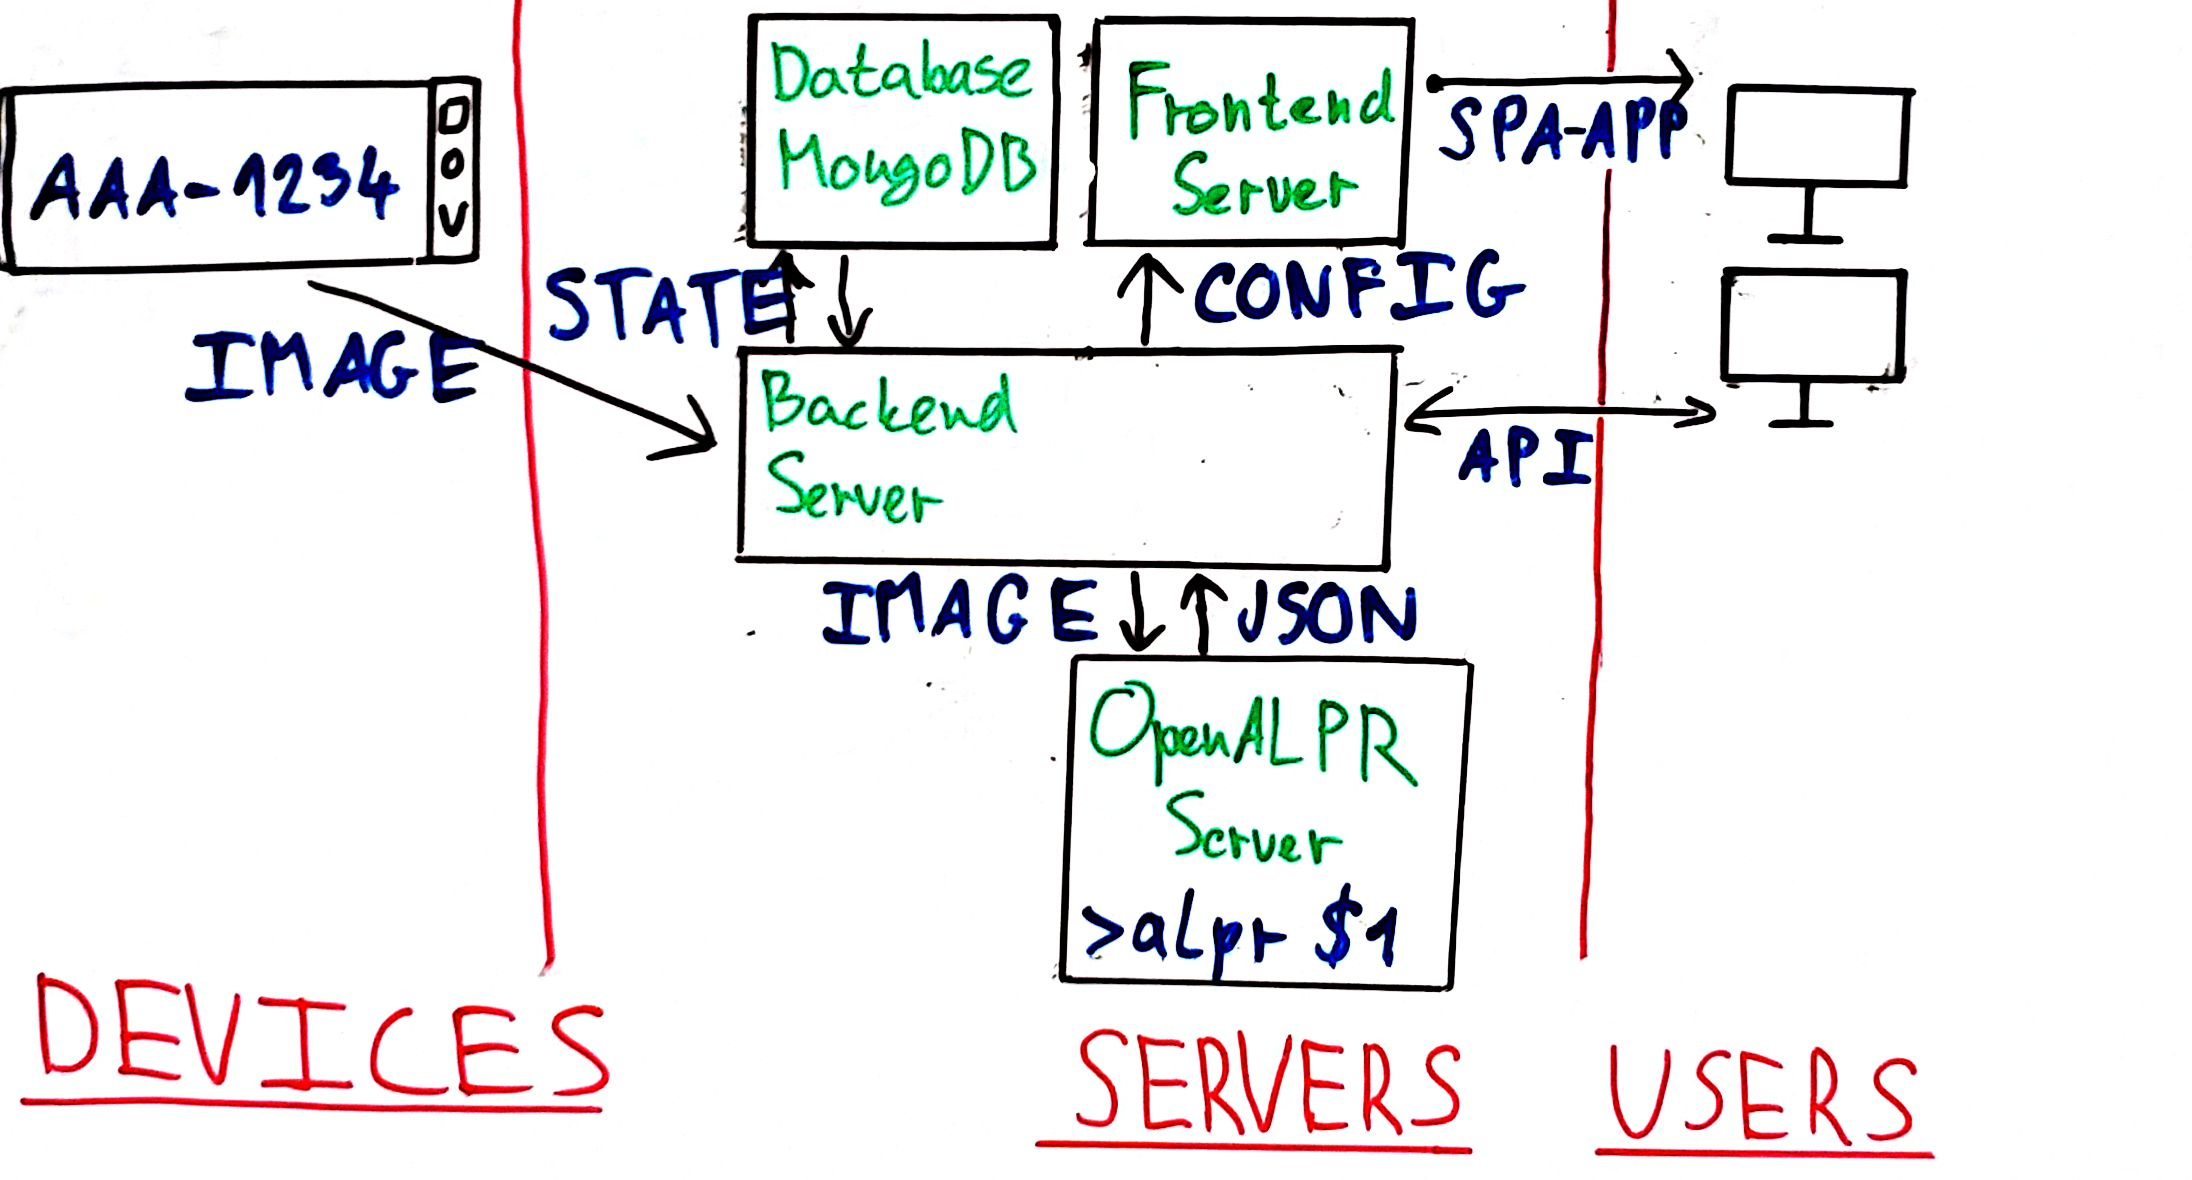
\includegraphics[width=145mm]{../img/architecture_drawing.jpg}
  \caption{Diagram komponent a jejich komunikace.}
  \label{fig:architecture_drawing}
\end{figure}

Parkovací systém se zkládá z následujících částí, které si nyní popíšeme stručně a detailněji později.
Části spolu komunikují pomocí HTTP.
Obrázek \ref{fig:architecture_drawing} ukazuje tyto části a nastiňuje způsob komunikace.

\begin{itemize}
  \item \textbf{Backend} je středobodem celé aplikace -- komunikuje se všemy ostatními komponentami.
        Zajišťuje business logiku aplikace, autentizaci i autorizaci uživatelů a perzistenci dat do \textbf{Databáze}.
  \begin{itemize}
    \item \textbf{Databáze} (nevlastní software -- https://www.mongodb.com/) k ukládání dat je MongoDB, která byla vybrána, protože data se budou
          převážně zapisovat a bude potřeba v nich rychle hledat a provádět agregační dotazy.
    \item \textbf{OpenALPR Server} (převzato z https://github.com/gerhardsletten/express-openalpr-server) je server, jenž obstarává přístup
          ke knihovně OpenALPR (https://github.com/openalpr/openalpr), která rozpoznává SPZ, přes protokol http.
  \end{itemize}
  \item \textbf{Mobilní aplikace} posílá obrazová data na \textbf{Backend}, kde jsou zpracována. Je určena pro platformu Android.
  \item \textbf{Frontend} je rozhraní mezi celým systémem a správcem parkoviště a dalšího personálu.
\end{itemize}

\section{Backend} \label{backend}

Jako programovací jazyk pro \textbf{Backend} byl zvolen staticky typovaný Typescript kvůli rychlosti vývoje
a množství knihoven, které poskytuje ekosystém Node.js.

\subsection{Autentizace a autorizace} \label{auther_authen}

Autentifikace lidských uživatelů bude probíhat pomocí standardního hesla a zařízení pomocí dlouhého, náhodně generovaného hesla,
které bude posíláno na Frontend ve formě QR kódu, které zařízení naskenuje.
TODO: Tokens

Autorizace pak bude probíhat bez Cookies, místo toho bude Access Token poslán v hlavičce HTTP hlavičce
\textit{Authorization}, čímž předejdeme CSRF/XSRF útokům.

\subsection{Komunikace s Frontendem}

Primárním způsobem komunikace s \textbf{Frontend}
je dotazovací jazyk GraphQL, který přináší ucelený popis poskytovanách dat pomocí kontroly typů,
expresivních dotazů, jejichž odpověď má stejný "tvar" v JSON formátu.
Obrázek \ref{fig:graphql_example} ukazuje dotaz hledání uživatele podle jména.

\begin{figure} \centering
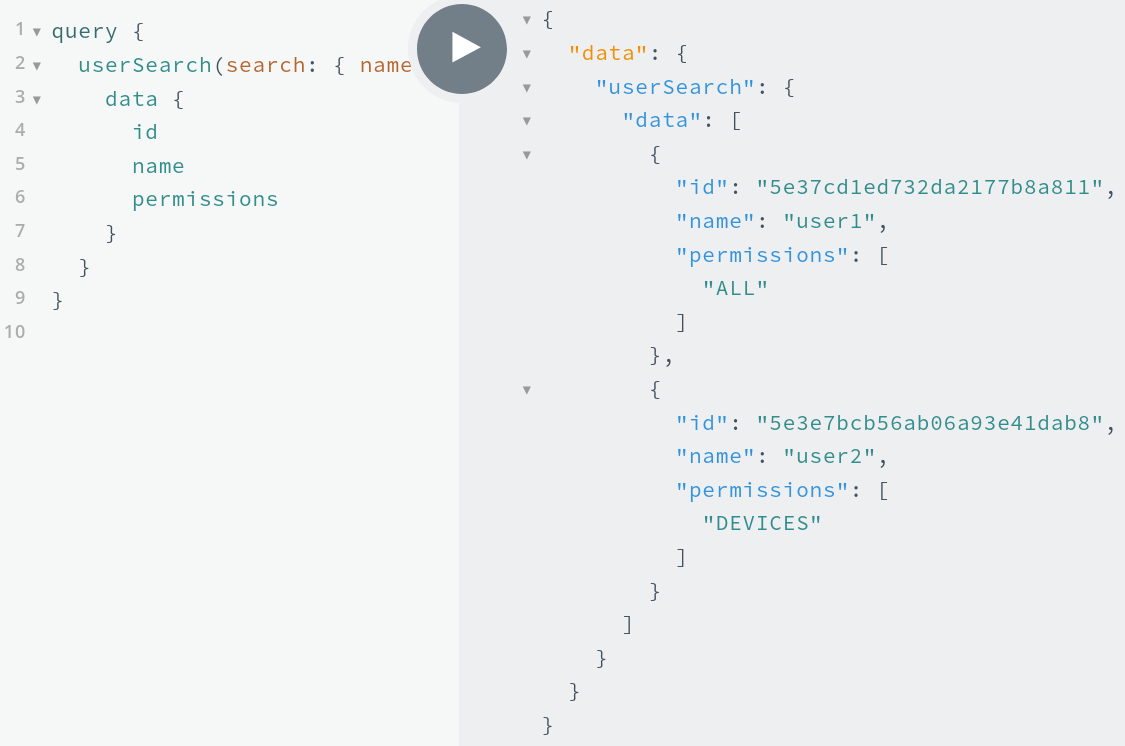
\includegraphics[width=145mm]{../img/graphql_example.png}
\caption{Příklad GraphQL dotazu (vlevo) a odpovědi (vpravo). Screenshot z nástroje GraphQL Playground.}
\label{fig:graphql_example}
\end{figure}

Model uživatele může mít i další atributy, ale GraphQL vrátí přesně ty údaje, na které se uživatel zeptal.
Tento triviální příklad neukazuje další funkce jako mutace dat, dědičnost typů, více dotazů v jednom http dotazu
a mnoho dalších.
GraphQL je pouze specifikace vytvořená společností Facebook. Detailní informace jsou dostupné na oficiálních
stránkach https://graphql.org/.

\subsection{Posílání obrázků}

Jelikož GraphQL posílá odpovědi v JSON, není vhodné na posílání obrázků. Je to možné za využití base64 kódování,
ale přes síť se přenese více bytů, než při použití obvyklého způsobu přes HTTP. Z toho důvodu pro posílání
obrázků (např. QR kódu pro Frontend pro autentifikace zařízení nebo zaznamenané znímky SPZ) bude mít Backend
klasické REST endpointy.

\section{Frontend} \label{frontend}

Pro \textbf{Frontend} byl jako u \textbf{Backend} vybrán Typescript ze stejných důvodů. Webové rozhraní
je takzvaná SPA (z angl. Single-Page-Application), což znamená, že uživateli se obsah mění dynamicky
bez načítání dalších stránek.
Renderování zajišťuje knihovna React, která od klasického přístupu, kdy se odděluje HTML a Javascript do separátních
souborů, mandatuje, že v jednom souboru je jedna komponenta se vším svým HTML a logikou ve formě Javascriptu nebo
Typescriptu. Pomocí další knihovny typestyle pak můžeme do stejného souboru psát i typované CSS.
Aby bylo možné snadno sdílet mezi komponentami stav, byla pro takzvaný state-management zvolena knihovna Redux.
Diagram na obrázku \ref{fig:react_redux_dataflow} ukazuje tok dat mezi Reactem a Reduxem.

Jelikož je aplikace vyvíjena pro správce systému a ne pro velké množství uživatelů, můžeme si dovolit
klást menší nároky na velikost aplikace (tj. můžeme přidávat i velké knihovny), což velice usnadní vývoj za
nízkou cenu.

\begin{figure}[!htb] \centering
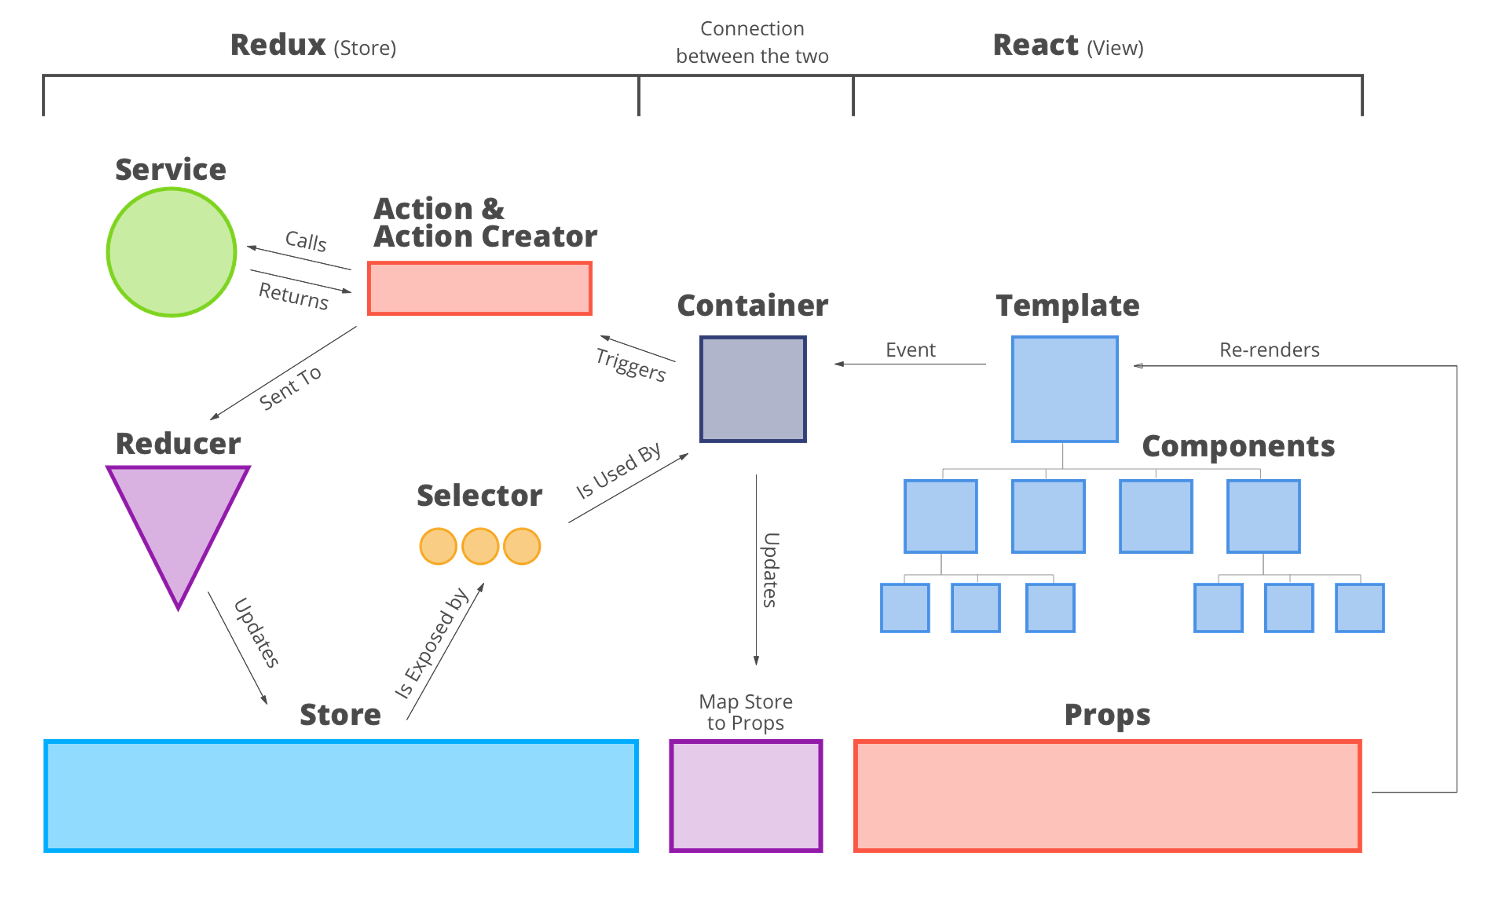
\includegraphics[width=145mm]{../img/react-redux-architecture.png}
\caption{Spojení React a Redux. \citep[viz][]{react_redux_dataflow}}
\label{fig:react_redux_dataflow}
\end{figure}

\subsection{Obrazovky}

Dle požadavků z úvodu mějme po příhlášení následující obrazovky, mezi kterými bude uživatel přepínat pomocí hlavního menu.

\begin{itemize}
  \item \textbf{Dashboard} -- jednoduché shrnutí nedávných statistik, kolik vozidel je
        momentálně na parkovišti, aktivní zařízení apod.
  \item \textbf{Statistiky} -- detailněji zobrazené údaje o počtu parkování a výdělku podle roku, měsíce a dne s grafy.
        Zde půjde i exportovat data to CSV souboru (\textit{Comma-Separated-Values}).
  \item \textbf{Pravidla a Filtry} -- definice parkovacích pravidel a filtrů vozidel (popsáno v \ref{analysis_parking_schema}).
        Pro ověření půjde si parkovací pravidla a filtry odsimulovat.
  \item \textbf{Zařízení} -- správa zařízení zachycujících fotografie SPZ, která lze autentifikovat do systému pomocí
        QR kódu.
  \item \textbf{Správa uživatelů} -- přidávání, odebírání a úprava uživatelů a jejich operávnění.
  \item \textbf{Správa účtu} -- změna údajů a hesla současně přihlášeného uživatele.
\end{itemize}

\section{Mobilní aplikce} \label{mobile_app}

\textbf{Mobilní aplikace}, která je určena pro platformu Android, měla volbu jazyka omezenou na Javu, Kotlin a C++.
Rychlost C++ není potřeba a navíc autor s tímto jazykem nižší úrovně nemá takové zkušenosti.
Kotlin oproti Javě umožňuje přímočarejší přístup k elementům uživatelského rozhraní, a proto byl zvolen.

Jediným úkolem \textbf{Mobilní aplikace} je v pravidelném intervalu pořídit snímek fotoaparátem a poslat ho na
\textbf{Backend}, který jej patřičně zpracuje.

% Maybe divide into smaller pieces

% Typescript
% - rychlost vývoje JS
% - type safety
% - Node ecosystem
%   - dev tools
%   - libraries
%   - npm
% - freedom of expression
% - scripts using main code

% VSCode
% - supports TS well
% - lightweight
% - plethora of extensions to ease development

% Docker for deployment

\section{Detekce SPZ}

Detekci SPZ bude zajišťovat knihovna OpenALPR \citep[viz][]{OpenALPR}, jejímž vstupem je obrázek a popřípadě
parametry jako úhel kamery apod. Ke zbytku aplikace je připojena malým HTTP serverem, jenž byl převzán a upraven
\citep[viz][]{OpenALPR_Server}.
Ten umožňuje poslat pomocí protokolu HTTP obrázek a obdržet JSON s SPZ daty a souřadnicemi detekované SPZ.
Samotný server ke knihovně přistupuje zavoláním binárky \textit{alpr}, který jako argument přijme cestu k
obrázku, ve kterém hledáme SPZ. Alternativní a lepší způsob přístupu by bylo mít v Node.js přímo takzv.
\textit{language-binding}, ale to se autorovi (a mnoho dalším, kteří se o to pokoušeli) nepodařilo.

% - just a phone taking photographs and analyzing them
%   - in the phone (rooted and/or with a normal Linux distro)
%   - remotely through back end
% - movement detection
% - size to filter distant vehicles that are not entering etc.

% - hash, salt
% - JWT
% - simple permission levels
%   - the system operates on its own most of the time
%   - many permissions and roles are confusing anyway

\section{Parkovací pravidla} \label{analysis_parking_schema}

\begin{itemize}
  \item Různá vozidla mohou podléhat ruzným pravidlům.
  \item Pravidla mají prioritu.
  \item Pravidla mají časové omezení.
  \item V jednu chvíli může platit více pravidel.
\end{itemize}

Mechanismus, kterým umožníme vozidlům být ovlivněna některými pravidly,
budou filtry.
Pro dostatečnou flexibilitu je zapotřebí oddělit samotná pravidla od jejich
priority, časového intervalu platnosti i filtrů,
k čemuž bude sloužit objekt typu \texttt{ParkingRuleAssignment}.

% TODO - add a db schema image that takes less space
\begin{lstlisting}
type ParkingRuleAssignment {
  rules: [ParkingRule]!
  start: DateTime!
  end: DateTime!
  # ALL nebo NONE
  vehicleFilterMode: VehicleFilterMode!
  vehicleFilters: [VehicleFilter!]
  priority: NonNegativeInt!
}

type VehicleFilter {
  id: ID!
  name: String!
  action: VehicleFilterAction!
  vehicles: [Vehicle!]!
}
\end{lstlisting}

Filtrování bude mít dva módy: začneme se všemi vozidly (ALL) a začneme bez vozidel (NONE).
Následné filtry mohou buď přidávat, nebo odstraňovat jednotlivá vozidla.
Hodí se mít filtry uložené separátně, aby mohli být využity několikrát.

Pro zjednodušení algoritmů, uvalíme omezení: ve stejný čas nesmí existovat více \texttt{ParkingRuleAssignment}
se stejnou prioritou.

\subsubsection*{Algoritmus filtru vozidel}

\textit{Vstup: objekt \texttt{ParkingRuleAssignment}, vozidlo}

\textit{Výstup: boolean určující platnost}
\begin{enumerate}
  \item Na základě módu filtrování si budeme udržovat množinu buď odstraněných vozidel (mód ALL), nebo přidaných vozidel (mód NONE).
  \item Podle příslušné akce filtrů (odstranit nebo přidat) budeme množinu našich vozidel manipulovat. Např. je-li mód ALL a filtr odstraňuje, do množiny si vozidla přidáme.
  \item Pokud je vozidlo ve výsledné množině, tak pro něj \texttt{ParkingRuleAssignment} platí pokud je filtrovací mód NONE a neplatí pokud je mód ALL. Opačné výsledky nastanou, pokud vozidlo v množině není.
\end{enumerate}

Časová i paměťová složitost algoritmu je ${\cal O}(N)$, kde $N$ je počet filtrů.

Tento algoritmus lze potenciálně rozdělit na předvýpočet (kroky 1. a 2.) a ověření (krok 3.).
To je jedna možnost, která zvýší paměťovou náročnost, protože bychom si museli pamatovat množiny, což je nepraktické.
Je-li uživatel příčetný, počet použitých filtrů nebude obrovský, a tudíž je lepší zvolit následující způsob cachovaní.
Zapamatujeme si výsledky pro určitý seznam filtrů pro konkrétní vozidlo pouze při běhu algoritmu, který je
vysvětlen v následující kapitole, čímž následující algoritmus zrychlíme.

\subsubsection*{Algoritmus pro aplikaci ParkingRuleAssignmentů}

\begin{figure}[!htb] \centering
  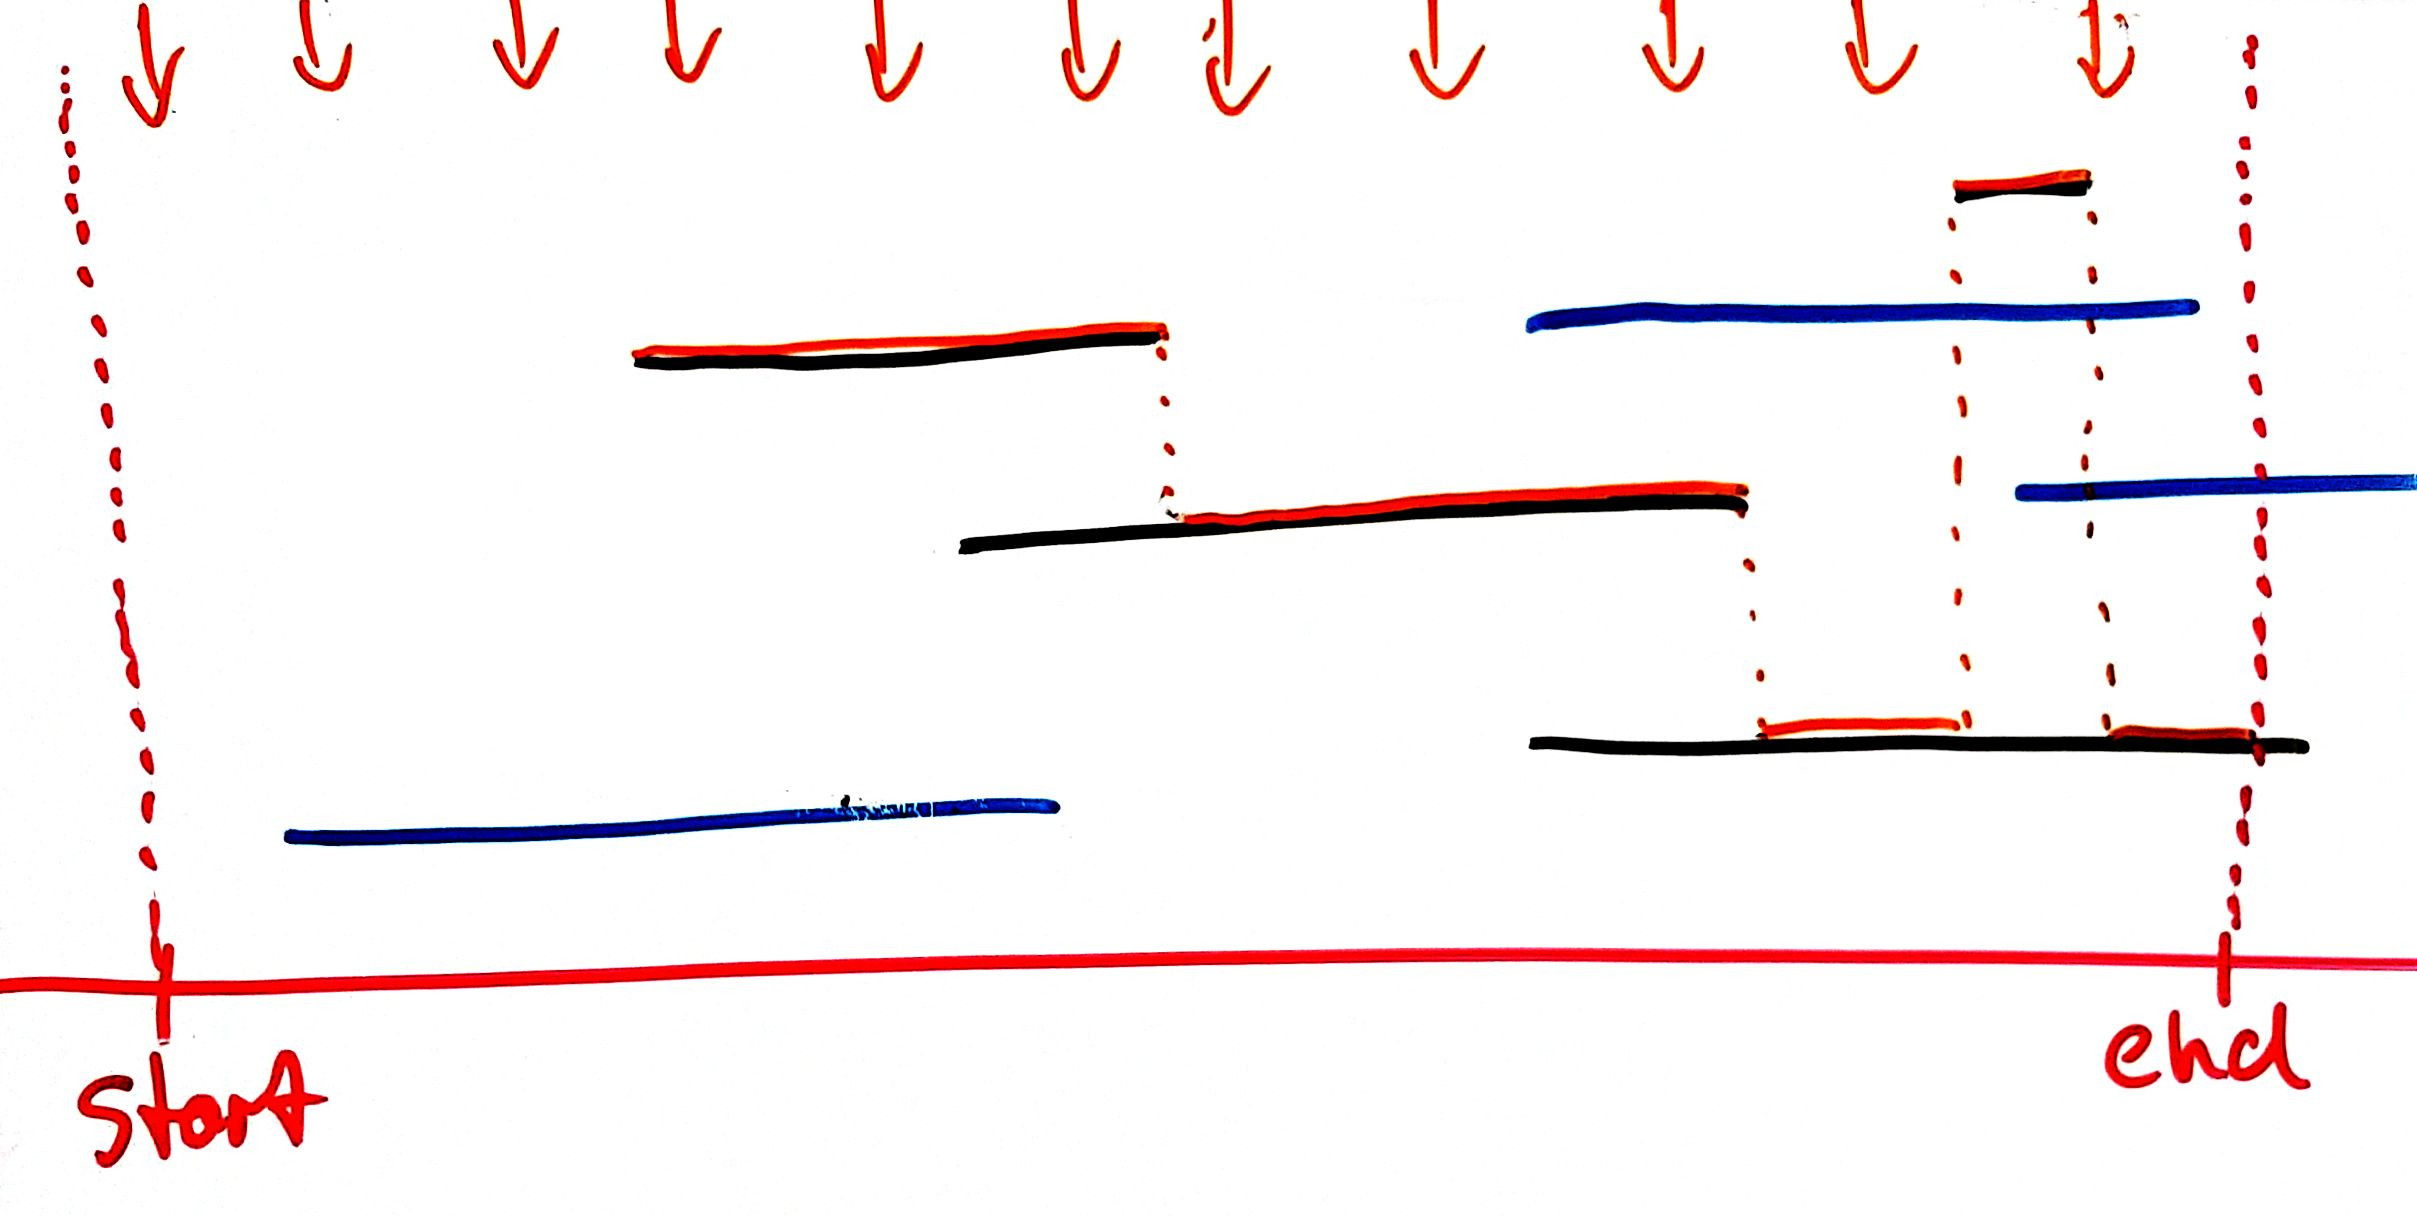
\includegraphics[width=145mm]{../img/rules_drawing.jpg}
  \textit{Modré úsečky neplatí kvůli filtrům nebo protože jsou deaktivované. Oranžová čára značí výstup požadovaného algoritmu.}
  \caption{Ilustrace problému úseček. }
  \label{fig:rules_drawing}
\end{figure}

V jednom čase může existovat více objektů typu \texttt{ParkingRuleAssignment} avšak s různou prioritou.
Může se stát, že aplikovaných \texttt{ParkingRuleAssignment} bude několik (různé priority, vyprší platnost, etc.).

Situaci si lze představit jako několik úseček navzájem rovnoběžných úseček v různých výškách, které se neprotínají.
Nás nyní zajímá, na které a v jakých intervalech na ně dopadne světlo, pokud na ně kolmo zeshora posvítíme.
Situaci lze vidět na obrázku \ref{fig:rules_drawing}.

Pro zjednodušení předpokládejme, že všechny \texttt{ParkingRuleAssignment}, které zpracováváme, platí pro naše vozidlo.
Přidat tuto kontrolu později je triviální.

\textit{Vstup: seznam \texttt{ParkingRuleAssignmentů} odpovídající pro interval pobytu vozidla na parkovišti, vozidlo}

\textit{Výstup: seznam \texttt{ParkingRuleAssignmentů} s časy platnosti}
\begin{enumerate}
  \item Seřadíme si začátky a konce úseček podle jejich času.
  \item Vytvoříme si haldu pro odkládání úseček, která řadí podle priority -- větší výše.
  \item Vytvoříme si seznam aplikovaných pravidel s časy (časy mohou se lišit od počátečních i koncových časů).
  \item Nechť \textit{s} je současná úsečka a \textit{$t_s$} čas zvolení \textit{s} (čas zvolení se může lišit od začátku úsečky).
  \item Pro každou událost \textit{u} značící začátek/konec úsečky (aplikaci pravidla) \textit{p}:
  \begin{enumerate}
    \item Pokud se jedná o začátek nové úsečky:
    \begin{enumerate}
      \item Pokud není zvolená úsečka:\\
            \textit{$t_s$} $\leftarrow$ \textit{p.start}\\
            \textit{s} $\leftarrow$ \textit{p}
      \item Pokud je zvolená úsečka a \textit{p} má vyšší prioritu než \textit{s}:\\
            \textit{s} dáme do seznamu aplikovaných pravidel se začátkem \textit{$t_s$} a koncem \textit{p.start}.\\
            \textit{s} dáme na haldu, pokud \textit{s.end} > \textit{p.end}.\\
            \textit{$t_s$} $\leftarrow$ \textit{p.start}\\
            \textit{s} $\leftarrow$ \textit{p}
      \item Pokud je zvolená úsečka a \textit{p} má nižší prioritu než \textit{s} a \textit{p.end} > \textit{s.end}:\\
            \textit{s} dáme na haldu
    \end{enumerate}
    \item Jinak (jedná se o konec nějaké úsečky):
    \begin{enumerate}
      \item Přidáme \textit{s} do seznamu aplikovaných pravidel se začátkem \textit{$t_s$} a koncem \textit{s.end}.
      \item Taháme z haldy, dokud nedostaneme úsečku s koncem později než konecm \textit{p}, nebo dokud halda není prázdná.
      \item Pokud jsme z haldy vhodnou úsečku vytáhli, použijeme ji. V opačném případě vyprázdníme \textit{s} a \textit{$t_s$}.
    \end{enumerate}
  \end{enumerate}
\end{enumerate}

Agloritmus zajisté doběhne, protože máme konečný počet událostí a v každém cyklu jednu zpracujeme.
Při rozumném počtu \texttt{ParkingRuleAssignment} v daném intervalu je algoritmus velice rychlý.
${\cal O}(N^2\cdot logN)$
${\cal O}(N\cdot logN)$
Přidáme-li filtrování, které nemusíme provést pro všechny úsečky, ${\cal O}(N\cdot M)$.

\section{Databázové schéma} \label{db_schema}


\chapter{Předběžné testování rozpoznání SPZ} \label{proof_of_concept}


% TODO: Mby call it Vývojová dokumentace
\chapter{Vývoj} \label{vyvoj}

% Zakladni funkcionalita
% - BE -> Login, Tokens, Securing endpoints and GQL (with depth)
% - FE -> Menu, Page switching

% - BE -> GQL -> Optimizations, DI
% - SC -> Send images

% - FE -> Transferred size if compressed and if not compressed

% Problems
% - SC -> Keep capturing -> keep screen on which is not suitable for devices with an OLED



\chapter{Uživalteská dokumentace} \label{uzivatelska_dokumentace}

%%% Fiktivní kapitola s ukázkami sazby

\chapter{Kapitola} \label{kapitola1}

<Content>

\citep[viz][]{examplecit}


\chapter*{Závěr}
\addcontentsline{toc}{chapter}{Závěr}

Výsledný projekt splňuje celé zádání kromě jednoho bodu -- konkrétně se jedná o
různý provoz
o svátích a podobných dnech (viz \ref{missing1}). Implementace takovéto funkcionality
vyžaduje implementovat kalendář.
Co se týče rozpoznávání SPZ, statistik, samotných pravidel a filtrů vozidel,
tak zde je vše implementováno a funguje skvěle.
Při prohlížení záznamů parkování lze nahlédnout na výřez SPZ z pořízeného snímku.
Navíc lze pravidla a filtry simulovat pro libovolné vozidlo.

Vývoj byl díky vhodně zvoleným technologiím poměrně rychlý a bezbolestný.
V jeho průběhu nedošlo k žádnému backtrackování kvůli předchozím rozhodnutím.
Projekt je bez velkých obtíží rozšiřitelný a pozměnitelný.
Dalším rozšířením, aby projekt byl plnohodnotný parkovací systém, by byla
integrace s platebním terminálem a závorou.


%%% Seznam použité literatury
%%% Seznam použité literatury (bibliografie)
%%%
%%% Pro vytváření bibliografie používáme bibTeX. Ten zpracovává
%%% citace v textu (např. makro \cite{...}) a vyhledává k nim literaturu
%%% v souboru literatura.bib.
%%%
%%% Příkaz \bibliographystyle určuje, jakým stylem budou citovány odkazy
%%% v textu. V závorce je název zvoleného souboru .bst. Styly plainnat
%%% a unsrt jsou standardní součástí latexových distribucí. Styl czplainnat
%%% je dodáván s touto šablonou a bibTeX ho hledá v aktuálním adresáři.

\bibliographystyle{czplainnat}    %% Autor (rok) s českými spojkami
% \bibliographystyle{plainnat}    %% Autor (rok) s anglickými spojkami
% \bibliographystyle{unsrt}       %% [číslo]

\renewcommand{\bibname}{Seznam použité literatury}

%%% Vytvoření seznamu literatury. Pozor, pokud jste necitovali ani jednu
%%% položku, seznam se automaticky vynechá.

\bibliography{literatura}

%%% Kdybyste chtěli bibliografii vytvářet ručně (bez bibTeXu), lze to udělat
%%% následovně. V takovém případě se řiďte normou ISO 690 a zvyklostmi v oboru.

% \begin{thebibliography}{99}
%
% \bibitem{lamport94}
%   {\sc Lamport,} Leslie.
%   \emph{\LaTeX: A Document Preparation System}.
%   2. vydání.
%   Massachusetts: Addison Wesley, 1994.
%   ISBN 0-201-52983-1.
%
% \end{thebibliography}


%%% Obrázky v bakalářské práci
%%% (pokud jich je malé množství, obvykle není třeba seznam uvádět)
\listoffigures

%%% Tabulky v bakalářské práci (opět nemusí být nutné uvádět)
%%% U matematických prací může být lepší přemístit seznam tabulek na začátek práce.
\listoftables

%%% Použité zkratky v bakalářské práci (opět nemusí být nutné uvádět)
%%% U matematických prací může být lepší přemístit seznam zkratek na začátek práce.
% \chapwithtoc{Seznam použitých zkratek}

%%% Přílohy k bakalářské práci, existují-li. Každá příloha musí být alespoň jednou
%%% odkazována z vlastního textu práce. Přílohy se číslují.
%%%
%%% Do tištěné verze se spíše hodí přílohy, které lze číst a prohlížet (dodatečné
%%% tabulky a grafy, různé textové doplňky, ukázky výstupů z počítačových programů,
%%% apod.). Do elektronické verze se hodí přílohy, které budou spíše používány
%%% v elektronické podobě než čteny (zdrojové kódy programů, datové soubory,
%%% interaktivní grafy apod.). Elektronické přílohy se nahrávají do SISu a lze
%%% je také do práce vložit na CD/DVD. Povolené formáty souborů specifikuje
%%% opatření rektora č. 72/2017.
% \appendix
% \chapter{Přílohy}

% \openright
\end{document}
